\chapter{Formal Analysis}
In this chapter we will formally analyze our representation of the world as
described in Figure \ref{fig:classDiagram} using the Alloy language. Firstly we
define all the entities that populate the world, then we specify a set of
constraints that keep the representation coherent. Lastly we define some
functions that allow to see some properties of the model.

\section{Entities definition}
<<<<<<< HEAD
\lstinputlisting[language=alloy, firstline=1, lastline=53]{alloy/model.als}
=======
Here are defined all the entities we need for the formal analysis.
\begin{alloy}
sig Username, Password {}

abstract sig Person {
    username : one Username,
    password : one Password
}

sig FiscalCode{}

sig User extends Person {
    id : one FiscalCode
}

sig Operator extends Person {}

sig Municipality {}

sig Authority {
    employs : some Operator,
    zone : some Municipality
}

sig Vehicle {
    plate : one LicensePlate
}

sig LicensePlate {}

sig Violation {
    where : one Location,
    vehicle : one Vehicle,
    picture : one Picture
}

sig Picture{}

sig Location {
    belongsTo : one Municipality,
    latitude : one Int,
    longitude : one Int
}{
    latitude > -90 and latitude < 90 and
    longitude > -180 and longitude < 180
}

sig Accident{
    crashWhere : one Location
}

sig SuggestedAction {
    possibleCause : some Violation,
    prevents : some Accident
}
\end{alloy}
>>>>>>> 935d5d3757ccc180dda5c4e1d01301385681f6ce

\section{Constraints}
Here are defined all the constraints needed to keep the model coherent. The
majority of these are called \emph{noFoster[...]} and the name self describes
what the constraint does: we do no want usernames or passwords without their own
owner, same for pictures without their own violation, license plate without vehicle
and so on.

The second set of constraint defines the uniqueness of some entities, for
example there cannot be two different people with the same fiscal code or two
vehicles with the same license plate. These are constraints that are needed due
to real world limitations, but similar constraints are defined for entities not
present in the real world, for example \emph{Username}, which has to be unique
only due to our model design.

\begin{alloy}
    fact noFosterFiscalCode {
        all fisc : FiscalCode | fisc in User.id
    }

    fact noFosterPassword {
        all p : Password | p in Person.password
    }

    fact noFosterUsername {
        all u : Username | u in Person.username
    }

    fact noFosterOperator {
        all op : Operator | op in Authority.employs
    }

    fact noFosterMunicipality {
        all mun : Municipality | mun in Authority.zone
    }

    fact noFosterVehicles {
        all v : Vehicle | v in Violation.vehicle
    }

    fact noFosterLocation {
        all loc : Location | loc in Violation.where or loc in Accident.crashWhere
    }

    fact noFosterLicensePlate{
        all lp : LicensePlate | lp in Vehicle.plate
    }

    fact noFosterPicture{
        all pic : Picture | pic in Violation.picture
    }

    fact UniqueUsername {
        no disj a, b: Person | (a.username = b.username)
    } 

    fact noMultiJobs {
        all disj a, b : Authority | (no op : Operator | 
            op in a.employs and op in b.employs)
    }

    fact onlyOneAuthorityPerPlace {
        all disj a, b : Authority | (no mun : Municipality | 
            mun in a.zone and mun in b.zone)
    }

    fact UniqueLicensePlates {
        no disj v1, v2 : Vehicle | v1.plate = v2.plate
    }

    fact NoDuplicateLocations {
        no disj loc1, loc2 : Location | (loc1.latitude = loc2.latitude) or 
            (loc1.longitude = loc2.longitude)
    }

    fact UniquePictures {
        no disj v1, v2 : Violation | v1.picture = v2.picture
    }

    fact UniqueFiscalCode{
        no disj u1, u2 : User | u1.id = u2.id
    }
\end{alloy}
\section{Functions}
Here we describe a function that shows which \emph{Violations} are visible to
a certain \emph{Operator}. We make use of two auxiliary functions in order to
increase readability.
\lstinputlisting[language=alloy, firstline=122, lastline=132]{alloy/model.als}

\section{Generated Worlds}
With the following command we can generate some examples of the model we 
formalized.
\lstinputlisting[language=alloy, firstline=134, lastline=139]{alloy/model.als}
In particular we are asking the solver to have in our sample world at least 2
\emph{Operators}, 2 \emph{Users}, 2 \emph{Locations} and 2 \emph{Violations}.
Furthermore we are limiting the maximum cardinality for each entity at 4, and
the Integers in our model have a bitwidth of 9.

The output of the Alloy Analyzer for the previous command is the following:
\begin{lstlisting}
Executing "Run show for 4 but 9 int"
    Solver=sat4j Bitwidth=9 MaxSeq=4 SkolemDepth=1 Symmetry=20
    108896 vars. 4360 primary vars. 376105 clauses. 574ms.
    Instance found. Predicate is consistent. 1736ms.
\end{lstlisting}
and it shows that all the facts are consistent. The world generated with the
previous command is shown in figure \vref{fig:alloy_world}.

\begin{figure}[hb]
    \centering
    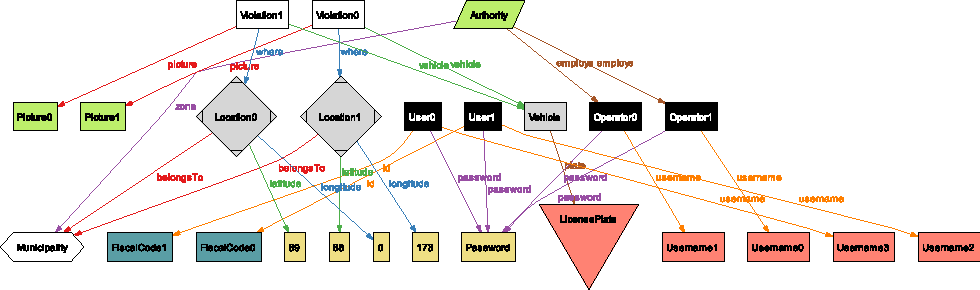
\includegraphics[width=\textwidth]{alloy_world}
    \caption{World generated from the Alloy model}
    \label{fig:alloy_world}
\end{figure}